%! TEX program = xelatex

\documentclass{beamer}
\setlength{\parindent}{0pt}
\setlength{\parskip}{1em}
\usepackage{fontspec}
\setmainfont{Lato}
\usepackage[english]{babel}

\usepackage{amsmath,amssymb,amsthm}
\usepackage{hyperref} % links
\usepackage{graphicx} % images
\usepackage{xcolor}

\definecolor{red}{HTML}{a20000}
\definecolor{green}{HTML}{306422}
\definecolor{blue}{HTML}{1d7d8e}

\newcommand{\img}[1]{
  \begin{center}
    \includegraphics[width=100pt]{#1}
  \end{center}
}


%
% begin document
%

% \usepackage[authordate,noibid,backend=biber]{biblatex-chicago}
% \addbibresource{}


\title{Diskreetti ulkoinen laskenta ja kontrollimenetelmä aikaharmonisessa akustiikkasimulaatiossa}
\author{Mikael Myyrä}
\date{Pro gradu -seminaari, kevät 2023}

\begin{document}

\frame{\titlepage}

\begin{frame}
  \frametitle{Akustiikkatehtävä}

  Mallinnetaan akustisia aaltoja: ääntä ja vastaavia ilmiöitä.
  Ratkaistavana aaltoyhtälö yhtälöryhmän muodossa:

  \[
    \begin{cases}
      \frac{\partial p}{\partial t} - c^2\nabla \cdot \mathbf{v} = f \\
      \frac{\partial \mathbf{v}}{\partial t} - \nabla p = 0 \\
    \end{cases}
  \]

  \pause

  jossa muuttujat
  \begin{itemize}
    \item $\mathbf{v}$: värähtelevien hiukkasten nopeus
    \item $p$: akustinen paine
  \end{itemize}

  (Ratkaisuun tarvitaan lisäksi alkutilanne ja reunaehdot)

  \pause

  \textbf{Jatkuva} malli
  $\rightarrow$ tietokoneella ratkaisu vaatii \textbf{diskretointia}
\end{frame}

\begin{frame}
  \frametitle{Diskreetti ulkoinen laskenta}

  Engl. \textit{Discrete Exterior Calculus} (DEC)

  JYU:n tieteellisen laskennan tutkimusryhmän aihe

  Esimerkkejä: \url{https://sites.google.com/jyu.fi/gfd}
\end{frame}

\begin{frame}
  \frametitle{Diskreetti ulkoinen laskenta}

  Rakennetaan kolmioverkko, joka peittää laskenta-alueen

  \img{dec_mesh_primal.pdf}

\end{frame}

\begin{frame}
  \frametitle{Diskreetti ulkoinen laskenta}

  Lisäksi \textit{duaaliverkko}, jossa jokaista ''primaaliverkon''
  tahkoa vastaa kärkipiste, kärkipistettä tahko,
  ja särmää kohtisuora särmä

  \img{dec_mesh_dual.pdf}

\end{frame}

\begin{frame}
  \frametitle{Diskreetti ulkoinen laskenta}

  Verkoissa on kolmen tyyppisiä elementtejä:
  \textcolor{red}{kärkipisteet}, \textcolor{green}{särmät} ja \textcolor{blue}{tahkot}

  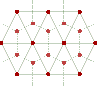
\includegraphics[width=0.3\textwidth]{dec_mesh_vertices.pdf}
  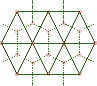
\includegraphics[width=0.3\textwidth]{dec_mesh_edges.pdf}
  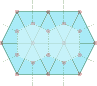
\includegraphics[width=0.3\textwidth]{dec_mesh_faces.pdf}
\end{frame}

\begin{frame}
  \frametitle{Diskreetti ulkoinen laskenta}

  DEC määrittelee elementtien välille suhteet:
  \begin{itemize}
    \item ulkoderivaatta $d$ siirtyy kärkipisteistä särmiin ja särmistä tahkoihin
    \item Hodgen tähti $\star$ siirtyy verkosta duaaliverkon vastaavaan elementtiin ja takaisin
  \end{itemize}

  \img{dec_operations.pdf}

  Näitä yhdistelemällä voidaan määritellä kaikki tehtävässä tarvittavat operaatiot,
  $\nabla = d$, $\nabla \cdot = d \star$
\end{frame}

\begin{frame}
  \frametitle{Kontrollimenetelmä}

  Ei tunneta alkutilannetta, vaan jokin muu ominaisuus.
  Etsitään alkutilanne joka toteuttaa ko. ominaisuuden
  
  \pause

  Tässä tapauksessa haluttu ominaisuus on aikaharmoninen tila:
  alkutilanne $u(0)$, josta aloittamalla
  simulaatio palaa samaan tilaan ajan $T$ kuluttua, $u(T) = u(0)$

  \pause

  Tämä on optimointitehtävä: minimoi $|u(T) - u(0)|$
  siten että $u$ toteuttaa aaltoyhtälön

  Voidaan käyttää tavallisiin optimointitehtäviin kehitettyjä algoritmeja!
\end{frame}

\begin{frame}
  \frametitle{Toteutus}

  Python-kirjasto PyDEC toteuttaa DEC:n perusoperaatiot

  gmsh -verkkogeneraattori rakentaa kolmioverkon

  Lähdekoodit GitHubissa: \url{https://github.com/m0lentum/decathlon} \\
  (huomaa käyttäjänimessä O:n paikalla nolla)
\end{frame}

\end{document}
